\documentclass[12pt, a4paper]{article}
\usepackage[utf8]{inputenc}

\usepackage{enumitem} 
\usepackage{graphicx} 
\usepackage{hyperref} 
\usepackage{etoolbox} 
\usepackage{float} 
\usepackage{titling} 
\usepackage{listings} 
\patchcmd{\thebibliography}{\section*{\refname}}{}{}{}
\graphicspath{{images/}} 

%\setlength{\droptitle}{-10em}   % This is your set screw

%\title{PROJECT REPORT \\ on \\[0.5in]\textbf{QUESTION ANSWERING SYSTEMS} \\[1in] Submitted in fulfilment of the course \\ \textbf{Study Oriented Project : CS F266} \\~\\ Submitted by \\ \textbf{Suchismita Tripathy : 2019A7PS0554P} \\~\\ Under the esteemed guidance and supervision of \\ \textbf{Mrs. L Rajya Lakshmi} \\Faculty, Department of Computer Science & Information Systems, \\ Birla Institute of Technology & Science, Pilani, 333031 Rajasthan, India 
% \author{Suchismita Tripathy \\ 2019A7PS0554P}
%\date{\vspace{-1.0cm}11 December 2021} 

%\usepackage{fancyhdr}
%\pagestyle{fancy}
%\fancyhf{}

\title{Online Question Answering System}
\author{Suchismita Tripathy}
\date{15 December 2021}

\begin{document}

\thispagestyle{empty} 
	
	\begin{center}
	
	\vspace{-2cm}
	\begin{figure}[h]
    
\includegraphics[scale=0.1]{bits logo.png} 
    \centering
	\end{figure}
	
	\vspace{0.8cm}
	\Large
	PROJECT REPORT 
	\\ on  
	
	\vspace{0.8cm}
	\LARGE
	\textbf{ONLINE QUESTION ANSWERING SYSTEMS}
	
	\vspace{1.3cm}	
	\Large
	Submitted in fulfilment of the course 
	\\ \textbf{Study Oriented Project : CS F266}

	\vspace{1cm}
	\large 
	Submitted by \\
	\Large
	\textbf{Suchismita Tripathy : 2019A7PS0554P}
	
	\vspace{1cm}
	\large
	Under the esteemed guidance and supervision of \\
	\Large
	\textbf{Mrs. L Rajya Lakshmi} \\
    \large
    Faculty, Department of Computer Science \& Information Systems, Birla Institute of Technology \& Science, Pilani, 333031 Rajasthan, India 
	
	\vspace{0.6cm}
	15 December, 2021
	\end{center} 

%\begin{document} 
%\maketitle 
\newpage
\section*{Acknowledgements}

I would like to take this opportunity to express my sincere gratitude to all the people who have supported me with this project, particularly Mrs. L Rajya Lakshmi without whom this project would not have been possible. Her guidance and support have been the key to the success of this project and her advice regarding the implementation helped me achieve increased accuracy and performance. 
\\~\\
I would also like to acknowledge the research done by Bolanle Ojokoh, Peter Ayokunle, Faisal Rahutomo, Teruaki Kitasuka, Masayoshi Aritsugi, Pranav Rajpurkar, Jiapeng Wang and Yihong Dong that greatly helped me complete the tasks for this project. 

\newpage 
\tableofcontents

\newpage 
\section{Introduction}

This project is focused on Question Answering systems and specifically, Community Question Answering or cQA systems. Question Answering is a subset of NLP and Information Retrieval that deals with the retrieval of answers to the questions provided as input by the user. This can take different forms, with the answers being retrieved from relevant documents or a corresponding extract or from a bank of already available question answer pairs. 
\\~\\
The questions provided as input may also take the form of definition questions, such as "Define binary search" or yes/no questions like "Is the Eiffel Tower in France?". These questions were not considered in this project as there are different ways of dealing with these that do not involve passage or question-answer pair retrieval (for eg: definition questions could be handled using frameworks like WordNet). Such questions will be handled only if they are already part of the datasets being used for cQA. 
\\~\\
Implementing a cQA system is the main aim of this project,. In order to gain some exposure to this field of NLP, I decided to focus on implementing a standard QA system for the first half of the semester. Thus I was able to learn about P.O.S. tagging, passage retrieval using cosine similarity and the general pipeline for such systems which was vital knowledge for the rest of the project. I then conducted further research and successfully implemented a cQA system. The evauation of the system is compared with the metrics and values achieved in the paper "Online Question Answering System" by Bolanle Ojokoh and Peter Ayokunle, which has been the main focus of this project. 
\\~\\ 
The project timeline is given on the following page.
\\~\\
\begin{figure}[h] 
    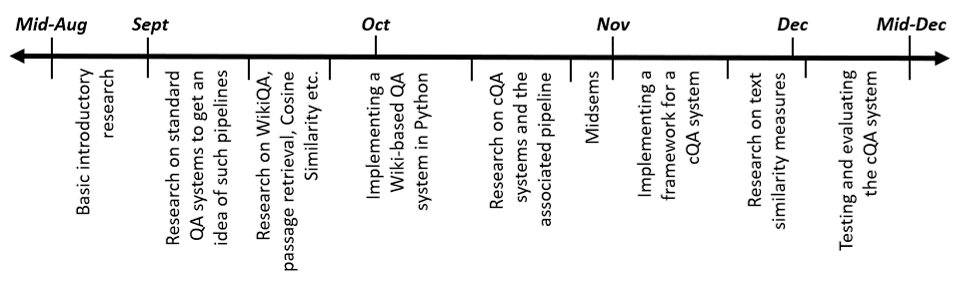
\includegraphics[scale=0.6]{timeline.png} 
    \centering 
    \caption{Project Timeline}
    \centering
\end{figure} 

\clearpage
\newpage 
\section{QA System Types} 

\subsection{Standard QA system based on passage retrieval} 
A QA system that does not rely on a pre-existing dataset of question-answer pairs like in cQA requires the implementation of document retrieval (unless all answers must be retrieved from only one given document) and passage retrieval as well, to find the right answer from the text that needs to be searched through. The general pipeline of the system would be as follows : 

\begin{enumerate}
    \item \textbf{Question Processing :} Clean and split question and retrieve relevant keywords using a P.O.S. tagger 
    \item \textbf{Document Retrieval :} Use keywords to search through a given set of documents and rank documents by their relation to the question (this could be done by comparing the question with the document titles) 
    \item \textbf{Passage Retrieval :} For the top or top few documents, extract the most relevant passages, using passage retrieval methods like Cosine Similarity, BM25 (that can also be used for document retrieval) and tools like Dense Passage Retrieval by HuggingFace 
    \item \textbf{Answer Retrieval :} For the top few retrieved passages, train a neural networks to use the question as a parameter and find the line from the passage that best answers the question 
    \item \textbf{Answer Ranking :} Rank the obtained answers by their confidence scores and return the first entry 
\end{enumerate}

\subsection{cQA System} 

Community Question Answering systems use datasets of questions that have already been provided by people in the past. These question-answer pairs are then compared to keywords each time a question is given as input. cQA systems are hence platforms where users' answers to questions are used. The advantages of cQA systems are : 

\begin{enumerate}
    \item Users' answers to questions keep adding to the dataset used by the system (auto-increasing dataset). 
    \item The system can thus give answers to questions itself when no users are available to answer. 
    \item The answers involved are given by actual humans and are hence near perfect as compared to answers derived from only documents or websites or a list of likely texts. 
    \item Since human answers are used, vague questions that are not fact based or require advice can also be answered by such systems. 
    \item System answers eliminate the time lag between a person asking a question and having to wait for a user who can answer to be available. 
\end{enumerate} 
\\~\\ 
The general pipeline is as follows : 

\begin{enumerate}
    \item \textbf{Question Processing :} Clean and split question and retrieve relevant keywords using a P.O.S. tagger 
    \item \textbf{Dataset Comparison :} Compare the given question with all the questions in the dataset using a suitable text similarity metric 
    \(\rightarrow\) A number of text similarity measure can be used for the same, and possible in conjunction
    \item \textbf{Question-Answer Pair Rating : } Rate the question-answer pairs for their relevancy to the input and return the most relevant one 
\end{enumerate}

\newpage 
\section{Stage I : Open-Domain Wiki QA System} 

\subsection{Tools/Theory} 
\subsubsection{MediaWiki API} 

The MediaWiki API is a web service by Wikipedia \cite{mediawiki} that allows access to features like authentication and search. It permits the user to access all the webpages of Wikipedia, across languages, look through the section titles and references and also access the images used. It thus enables the use of Wikipedia pages as a collection of documents. 
\\~\\ 
The API can be used with the following installation commands : 

\begin{lstlisting}[language = Python] 
!pip install wikipedia 
import wptools 
import wikipedia 
\end{lstlisting} 
\\~\\ 
The entire Wikipedia database can be searched through by using the wikipedia.search() function with keywords passed as parameters. Page IDs are used to access the different Wikipedia pages, passed as parameters to the wikipedia.page() function, which returns the entire contents of the page, though there are other functions that can be used to return only certain sections. 

\subsubsection{SQuAD 2.0} 

SQuAD or Stanford Question Answering Dataset is a dataset for reading comprehension and answer extraction. It includes groups of questions and paragraphs, a segment of which is the answer, whose location is defined by answer indices that are part of the dataset. The questions were posed by crowdworkers and the answers were derived from 365 of the top Wikipedia entries. \cite{squad} \cite{squadGit} Neural networks can be created and trained on this dataset to be able to identify sentences as answers from relevant passages in QA systems. Roberta Base is a machine learning model from HuggingFace that has been pretrained on the SQuAD 2.0 dataset, that can easily be imported into projects and used for answer exraction as part of QA pipelines. 

\subsubsection{Penn Treebank P.O.S. Tagger} 

P.O.S. Tagging or Part-Of-Speech Tagging is a staple process in NLP for classifying the words in a text into the different parts of speech like nouns, adjectives, adverbs etc. i.e. it involves tagging each word with its own lexical term. P.O.S. Tagging is implemented using hidden Markov models, unsupervised classification based on the contextx that different words occur in, dynamic programming methods etc. 
\\~\\ 
The Penn Treebank tagset is a list of part-of-speech tags that is widely used and based on English corpora. It has 36 P.O.S. tags and 12 others for punctuation. \cite{pos} The P.O.S. tags used for QA systems are generally, as presented in literature, adjectives, nouns, foreign words and proper nouns. 
\\~\\
As an example, for the question "Who played the Red Queen in Alice in Wonderland?", the tags are assigned as follows and 'Red', 'Queen', 'Alice' and 'Wonderland' are extracted as keywords : 

\begin{figure}[h]
    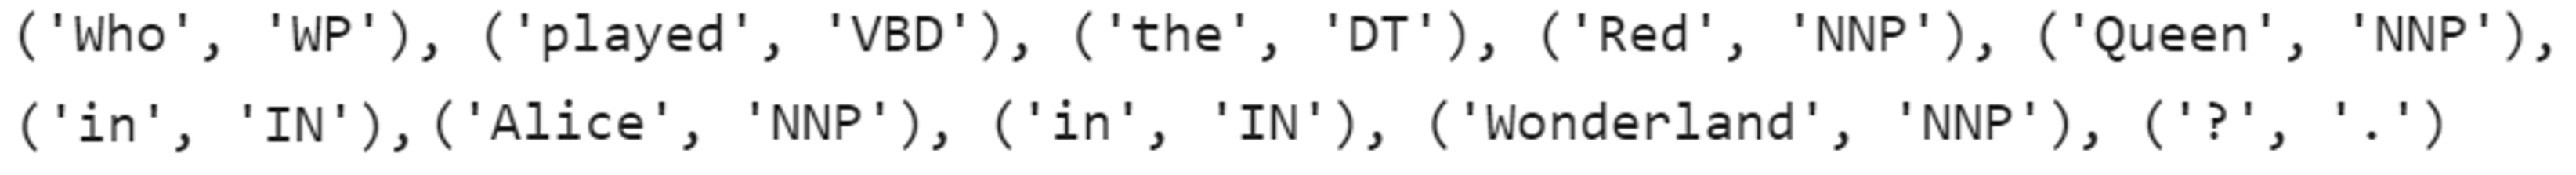
\includegraphics[scale=0.5]{pos tags eg.png} 
    \centering 
    \caption{P.O.S. Tags Example}
    \centering 
\end{figure} 

\begin{figure}[h]
    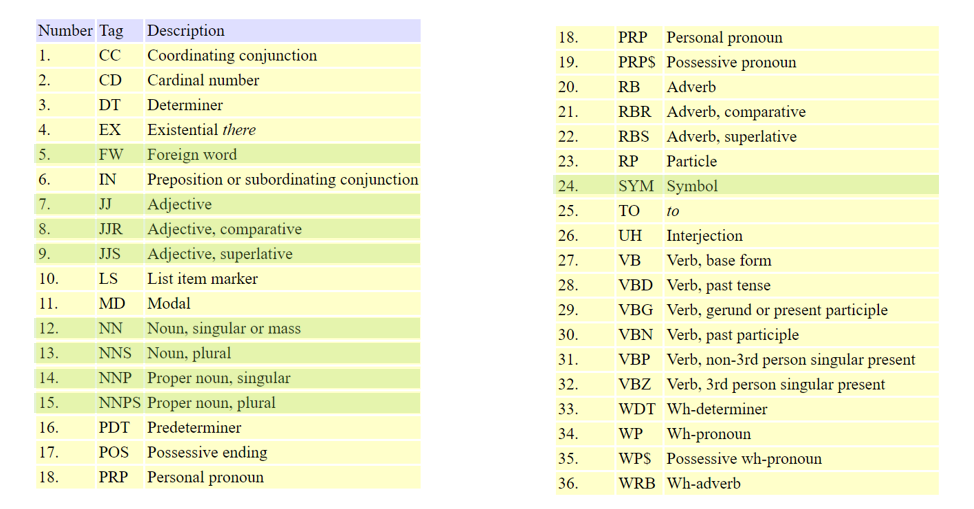
\includegraphics[scale=0.6]{pos stand.png} 
    \centering 
    \caption{Wiki QA P.O.S. Tags Used}
    \centering 
\end{figure} 

\subsubsection{Cosine Similarity} 

There are a number of other passage retrieval methods like BM25 and Dense Passage Retrieval by HuggingFace but Cosine Similarity was chosen for its ease of implementation and its high performance as indicated in the literature. 
\\~\\ 
Cosine similarity calculates similarity through the cosine of the angle between two vectors. \cite{cosine} \\ 
For two vectors \(X\) and \(Y\) where \\ 
\(X = (x_1, x_2, ..., x_n)\) and \(Y = (y_1, y_2, ..., y_n)\) 
\[|X| = \sqrt{x_1^2 + x_2^2 + ... + x_n^2}\]
\[|Y| = \sqrt{y_1^2 + y_2^2 + ... + y_n^2}\]
\\
\[X.Y = (x_1.y_1) + (x_2.y_2) + ... + (x_n.y_n)\]
\\ 
The similarity measure is thus 
\[similarity(X, Y) = \cos(\theta) = \frac{X.Y}{|X||Y|}\]
\\~\\
The similarity score is always between -1 and 1, as the range of natural values of \(\cos(\theta)\). If the vectors representing the sentences are aligned with \(\theta= 0^\circ\), the similarity measure is 1. If the vectors are orthogonal with \(\theta= 90^\circ\), the similarity measure is 0.  If the vectors are parallel but in opposite directions with \(\theta= 180^\circ\), the similarity measure is -1. 
\\~\\ 
To compare text through this measure, it is first required to get representations of the text extracts as vectors. This is done by building tf-idf document/passage vectors. A tf-idf vector for a word/term is proportional to term frequency and an inverse function of the number of documents in which it occurs. \cite{similarityMet} 
\[w_{i, j} = tf_{i, j} \log{\frac{N}{df_i}}\] 
\\
where \\  
\(w_{i,j}\) : weight of term \(i\) in document \(j\) \\ 
\(tf_{i, j}\) : term frequency of term \(i\) in document \(j\) \\  
\(N\) : number of documents in the corpus \\ 
\(df_i\) : number of documents containing term \(i\)  
\\~\\ 

The steps for the entire process using tf-idf vectorisation and calculation of cosine similarities are as follows : 

\begin{enumerate}
    \item \textbf{Modify array of passages :} Insert the base text that all other texts need to be compared to as the first entry of the array. 
    \item \textbf{Build tf-idf passage vectors :} Count features are extracted and tf-idf normalization and row-wise euclidean normalization are applied to generate tf-idf vectors using the TfidfVectorizer from the sklearn Feature Extraction library. 
    \item \textbf{Compute the dot product of the first row with the other rows :} To do this, either cosine\_similarity or linear\_kernel (which simply calculates dot products) from sklearn can be used. The magnitudes need to be taken into account but since row normalisation has already been carried out, the magnitudes are 1 and hence, linear\_kernel itself can be used. Both cosine\_similarity and linear\_kernel will give the same result but linear\_kernel takes less time to execute and performs better when a large amount of data is being handled. 
    \item \textbf{Sort the passages :} Sort the passages according to their cosine similarity with the first row of the array after removing the first element (this obviously has a cosine similarity of 1 as it has been compared with itself i.e. \(\theta = 0^\circ\)). 
\end{enumerate}

\subsection{Framework} 

The pipeline for the open-domain Wiki-based QA system implemented is shown here. The entire code can be found in the appendix in section 7.1. 

\clearpage 
\begin{figure}[h]
    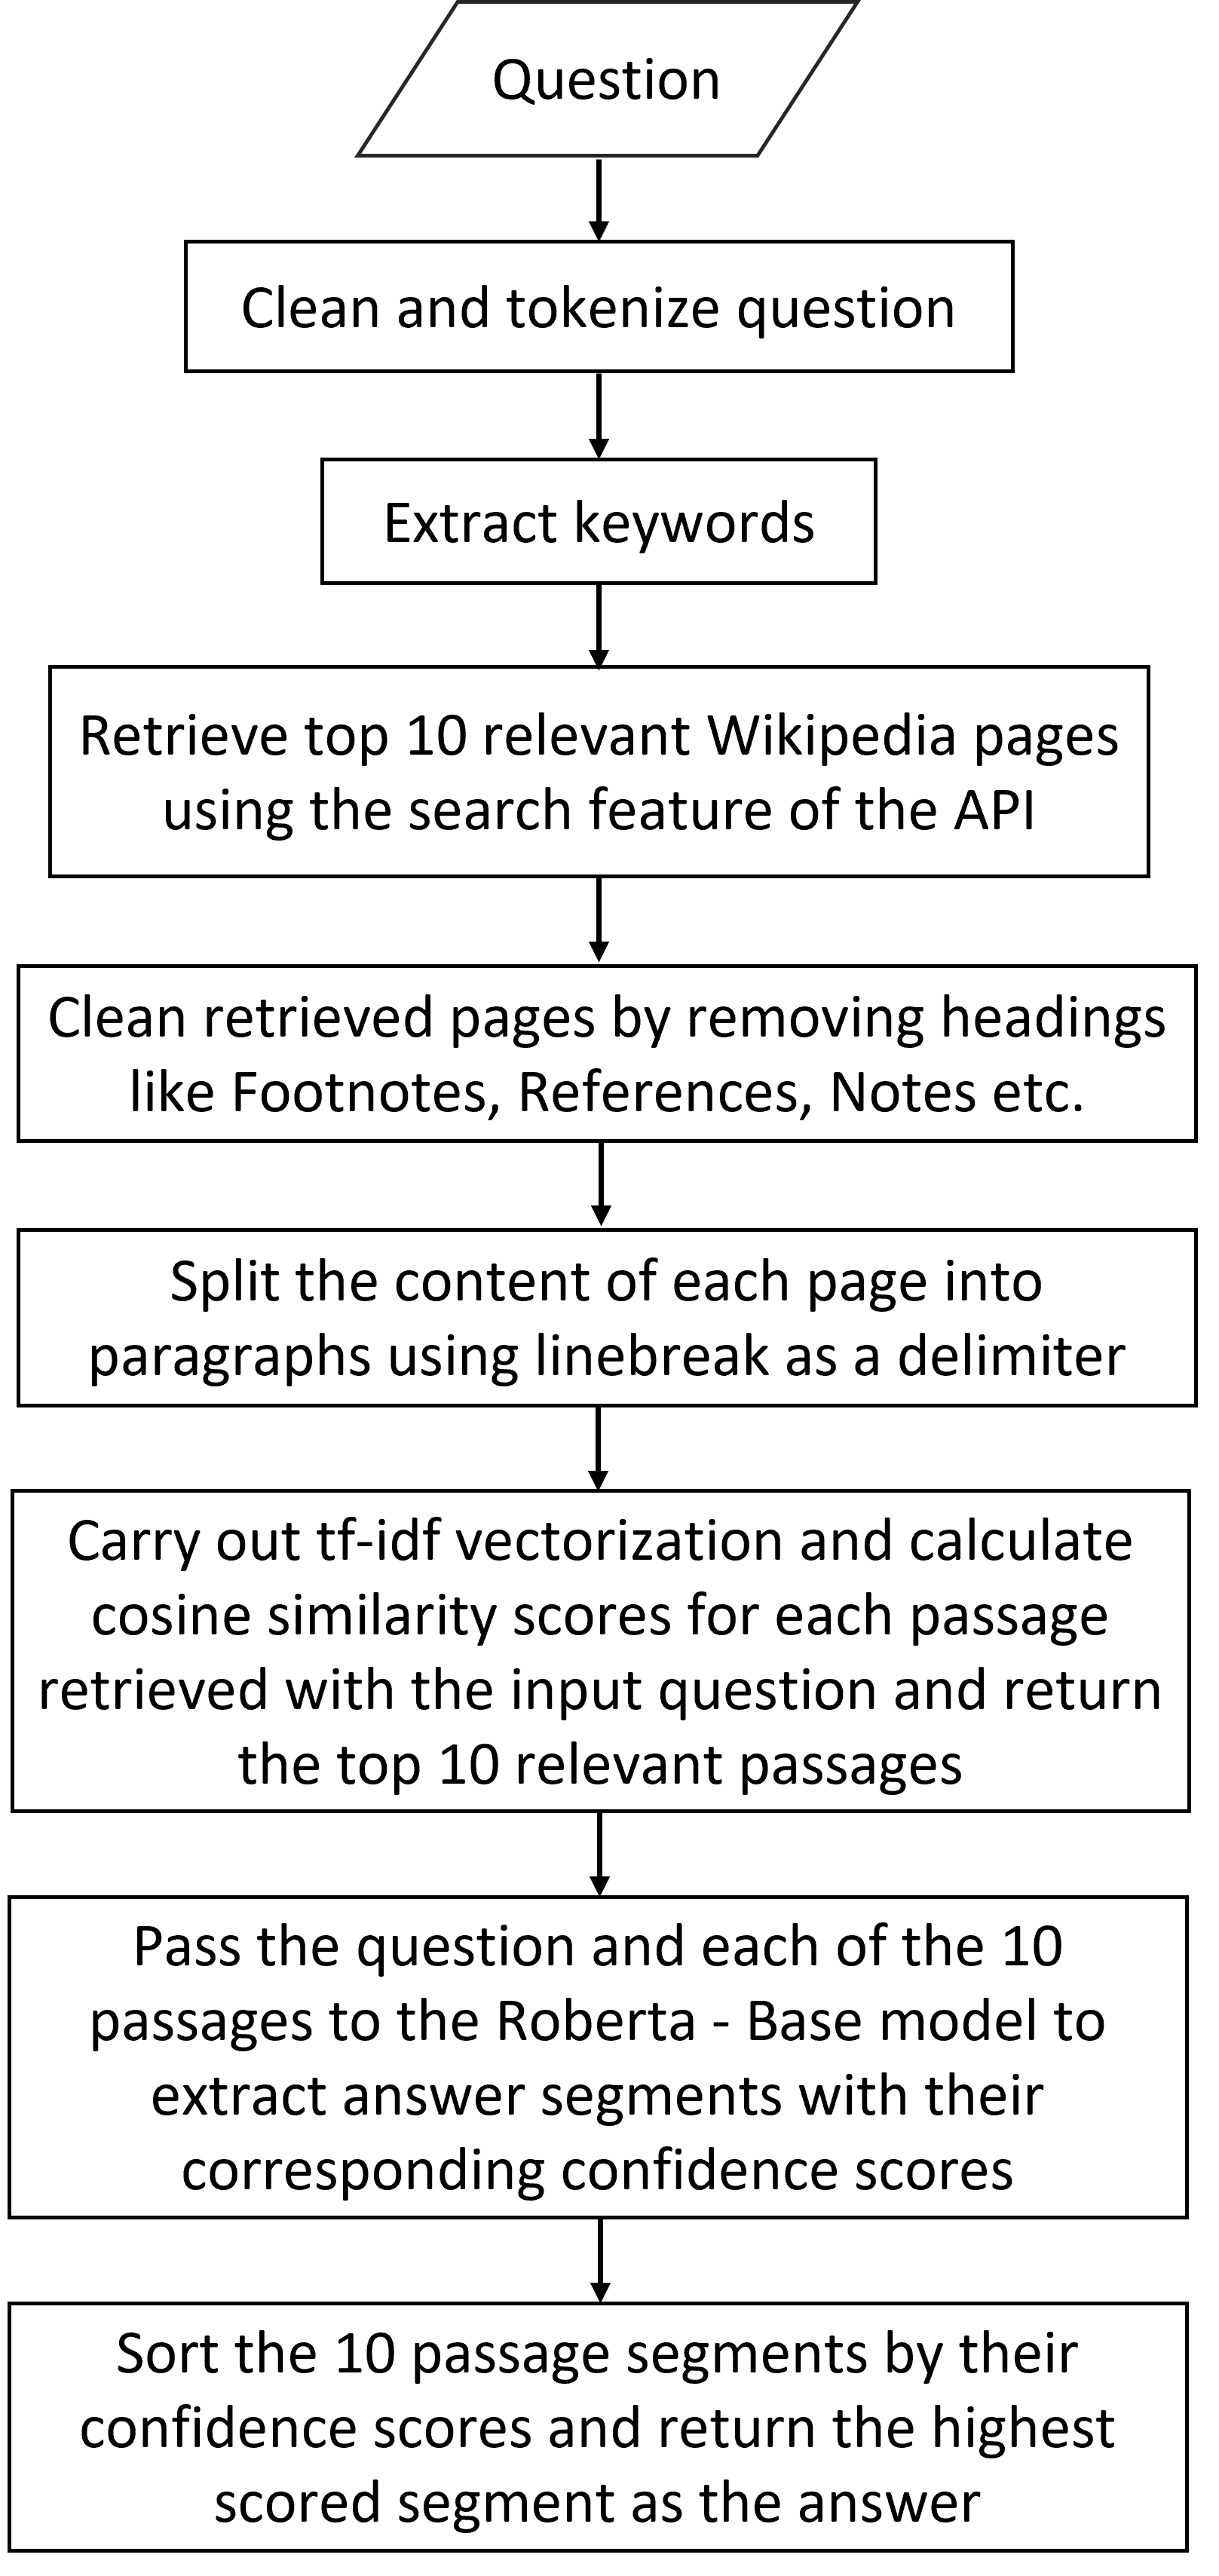
\includegraphics[scale=0.6]{wikiqa flowchart.png} 
    \centering 
    \caption{Wiki QA Pipeline}
    \centering 
\end{figure} 

\clearpage
\subsection{Performance} 

The system performs fairly well on most questions though its abilities are of course limited to the kind of information that is contained across Wikipedia pages : 

\begin{enumerate}
    \item Questions involving advice cannot be answered by such a system. 
    \item The system does not yet work for yes/no questions like "Is Australia a Continent?". 
    \item Example questions that work: What is the capital of Assam?, Who is the Greek goddess of Wisdom?, Where is Addis Ababa? 
    \item The system can be used for define questions. 
    \item Example questions that don't work: Who played Harley Quinn in the Suicide Squad?, What is a binary search tree? Who is the CEO of Apple? 
\end{enumerate} 

The system's performance can be considerably increased by trying different passage retrieval methods like BM25 and DPR, and finetuning and adding layers to the pretrained Roberta model used for answer extraction. \textbf{Since this was not the main focus of the project, more time was not spent on the WikiQA system since that would have led to less time spent on actually implementing and analysing the cQA system, though the improvements will be made in the future.}

\newpage 
\section{Stage II : cQA System} 

\subsection{Tools/Theory} 
\subsubsection{Penn Treebank P.O.S. Tagger} 

The tags that were used for keyword extraction for the cQA system are shown here \cite{pos}. In general, only foreign words, nouns, proper nouns and adjectives are used for the same but on running this on the question-answer pairs from the dataset, it was discovered that often words like "youtube" would not get recognised as belonging to one of these word classes and would instead get tagged as verbs. 

\begin{figure}[h]
    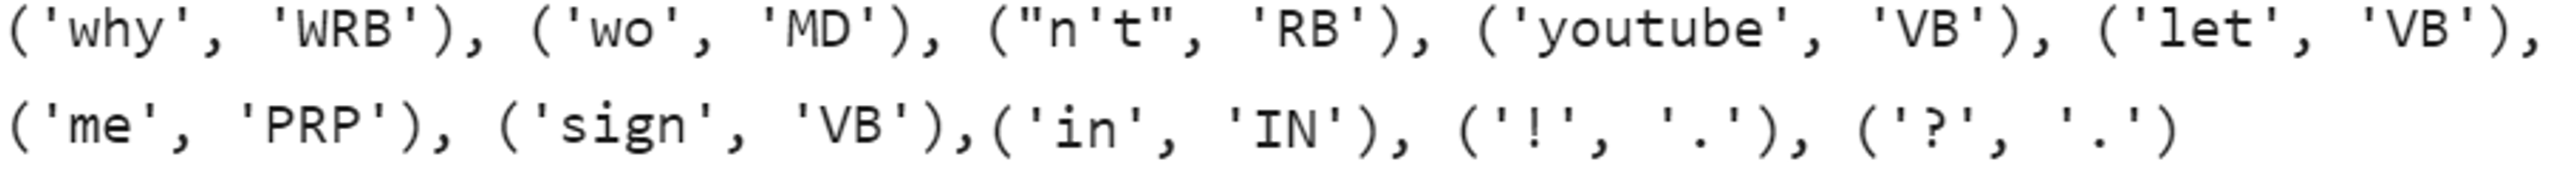
\includegraphics[scale=0.5]{pos tags youtube.png} 
    \centering 
    \caption{P.O.S. Tags generated for question "why won't youtube let me sign in!?"}
    \centering 
\end{figure} 

Hence, verbs were also considered in the system implemented and it was observed that this did not negatively the affect the system's performance on other question-answer pairs. 

\begin{figure}[h]
    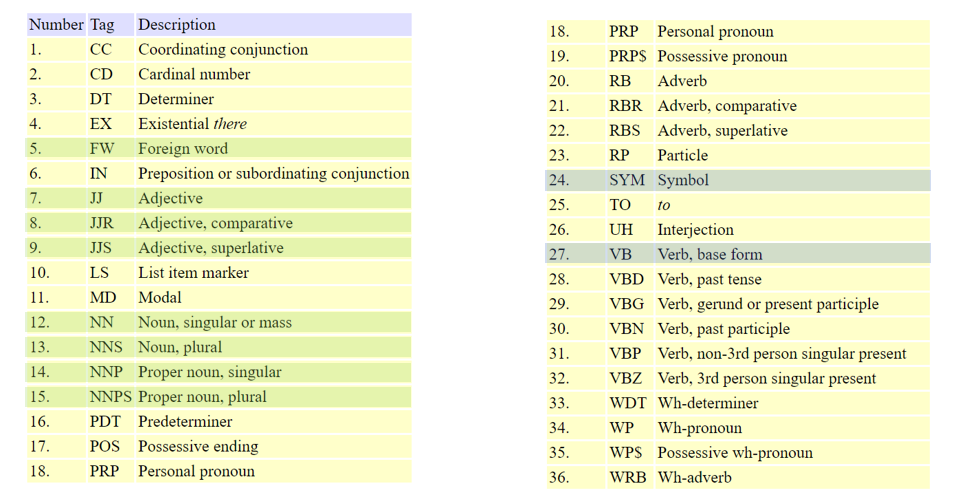
\includegraphics[scale=0.5]{pos cqa.png} 
    \centering 
    \caption{cQA P.O.S. Tags Used : Green indicates the tags suggested as important in the literature while Blue are those that were used in the current system in addition to the other tags}
    \centering 
\end{figure} 

\subsubsection{Dice Metric} 

The Dice Metric is one of the text similarity measures used commonly in QA systems. It is also often used, along with Jaccard scores, for evaluating segmentation performance for computer vision tasks. \cite{dice} The value of the metric depends on the number of shared words between the two texts being compared. 
\\~\\ 
Dice Metric = \(2 \times \frac{Number\; of\; words\; in\; A\cap B}{Length\; of\; A\; +\; Length\; of\; B}\)
\\~\\ 
The algorithm as presented in the literature \cite{maincqa} is as follows :

\begin{enumerate}
    \item  Get the two strings (say A and B) whose similarity is to be determined. 
    \item Extract keywords from string A. 
    \item Detect the number of keywords of A that are in B (i.e. A\(\cap\)B). 
    \item Multiply the result from step 3 by 2. 
    \item Determine the length of string A and B by counting the number of words in each. 
    \item Add the length of A and B together. 
    \item Divide the result from step 4 by the result from step 6. 
\end{enumerate}

\\~\\ 
The following is the pseudocode that was used to create an implementation of Dice Metric calculation based on the above algorithm : 

\begin{enumerate}
    \item Loop over the dataset. 
    \item Initialise a counter for each question subject to 0. 
    \item Loop over the keywords of the given question as returned by the P.O.S. tagger. 
    \item Increment the counter for each keyword that is part of the given question subject. 
    \item Multiply the above count by 2. 
    \item Divide the count by the sum of the lengths of the question and the current question subject. 
    \item Store the index of the question subject and the dice metric in a dictionary. 
    \item Sort the dictionary by value and return the 10 items with the highest dice metric values. 
\end{enumerate}

\subsubsection{Levenshtein Distance} 

Levenshtein Distance is another text similarity measure that depends on the number of shared words between the two texts being compared. Originally it is defined as the number of deletions, insertions or substitutions required to transform one string into another. This way, two strings are more similar if their Levenshtein Distance is lower, that two strings who have a higher Levenshtein Distance. \cite{levenshteinOrig} This algorithm uses characters as the base unit for comparisons. 
\\~\\ 
A modified version of Levenshtein distance that bases its comparisons of two strings on the number of shared words is a good alternative. It has been shown that the modified word-based version of the Levenshtein Distance \cite{maincqa} performs better than the original version for cQA and hence, this method was adopted for the system implemented for this project. 
\\~\\ 
Levenshtein Distance = \(Number\; of\; tokens\; in\; A\cap B\)
\\~\\ 
The algorithm as obtained from literature \cite{maincqa} is as follows : 

\begin{enumerate}
    \item Get the two strings (string1, string2) to compare.
    \item Split the two strings using a whitespace as delimiter (i.e. tokenize the two strings). 
    \item Remove any trailing “?”, “!”, “.” from the last word in both strings. 
    \item Store the tokens from both strings separately (i.e. tokensInString1, tokensInString2). 
    \item Loop through all elements in tokensInString1. 
    \item For each iteration in tokensInString1, test if a word (i.e. an element) is contained in tokensInString2. Also, test if the word is not a stopword (words which are filtered out prior to, or after, processing of natural language data (text)) 
    \begin{enumerate}
        \item If yes, increment a counter (initially set to zero) 
        \item Else do nothing and proceed to the next iteration 
    \end{enumerate} 
    \item At the end of the iteration, return counter. 
\end{enumerate}

\\~\\ 
The following is the pseudocode that was used to create the actual implementation of Levenshtein Distance calculation, based on the algorithm given above: 

\begin{enumerate}
    \item Clean the question by removing symbols and punctuation. 
    \item Tokenize the result by splitting the string with space as a delimiter. 
    \item Loop over the 10 indices with the highest dice metric values. 
    \item Similarly clean and tokenize the question subject under consideration. 
    \item Initialise a counter for each question subject to 0. 
    \item Loop over the tokens of the question. 
    \item Increment the counter for each token that is in the current question subject and is not a stop-word. 
    \item Multiply the edit distance with the corresponding dice metric value. 
    \item Store the index of the question subject and the above value in a dictionary. 
    \item Sort the dictionary and return the index with the highest metric. 
\end{enumerate}

\subsubsection{Cosine Similarity} 

In the search for other text similarity measures that could be implemented in an attempt to improve performance, I came across Jaccard Distance, and K Means (with word embeddings) \cite{textsims} along with Cosine Similarity \cite{similarityMet}, which is a text similarity measure in addition to a passage retrieval method. The literature seemed to suggest that cosine similarity would have the best performance among these 3 and hence I chose to implement this for the cQA system as I had done before for the Wiki QA system. The calculations are the same as presented before and the sklearn TfidfVectorizer was used for embeddings, with the linear\_kernel module to find cosine similarities. 

\subsection{Datasets} 
\subsubsection{Dataset 1 : Yahoo! Answers Dataset for cQA – 2010} 

The Yahoo! Answers Dataset - 2010 is a dataset of question-answer pairs from the popular platform Yahoo! Answers, divided into 3 categories : Internet, Hardware and Science. It was located and downloaded from SourceForge \cite{dataset1} as used in the literature \cite{maincqa}. The question-answer pairs from the topic 'Internet' were used and the split-up is as follows : 

\begin{center}
  \renewcommand{\arraystretch}{1.5}
  \begin{tabular}{c|c}
    Topic&Number of Questions\\ 
    \hline 
    Facebook&205\\ 
    Flickr&199\\ 
    Google&213\\ 
    MSN&199\\ 
    MySpace&192\\ 
    Wikipedia&201\\ 
    YouTube&198\\ 
    \hline 
    &1407
\end{tabular}
\end{center} 

The dataset contains the following files : 

\begin{enumerate}
    \item .xml files for each question 
    
    \begin{figure}[h]
        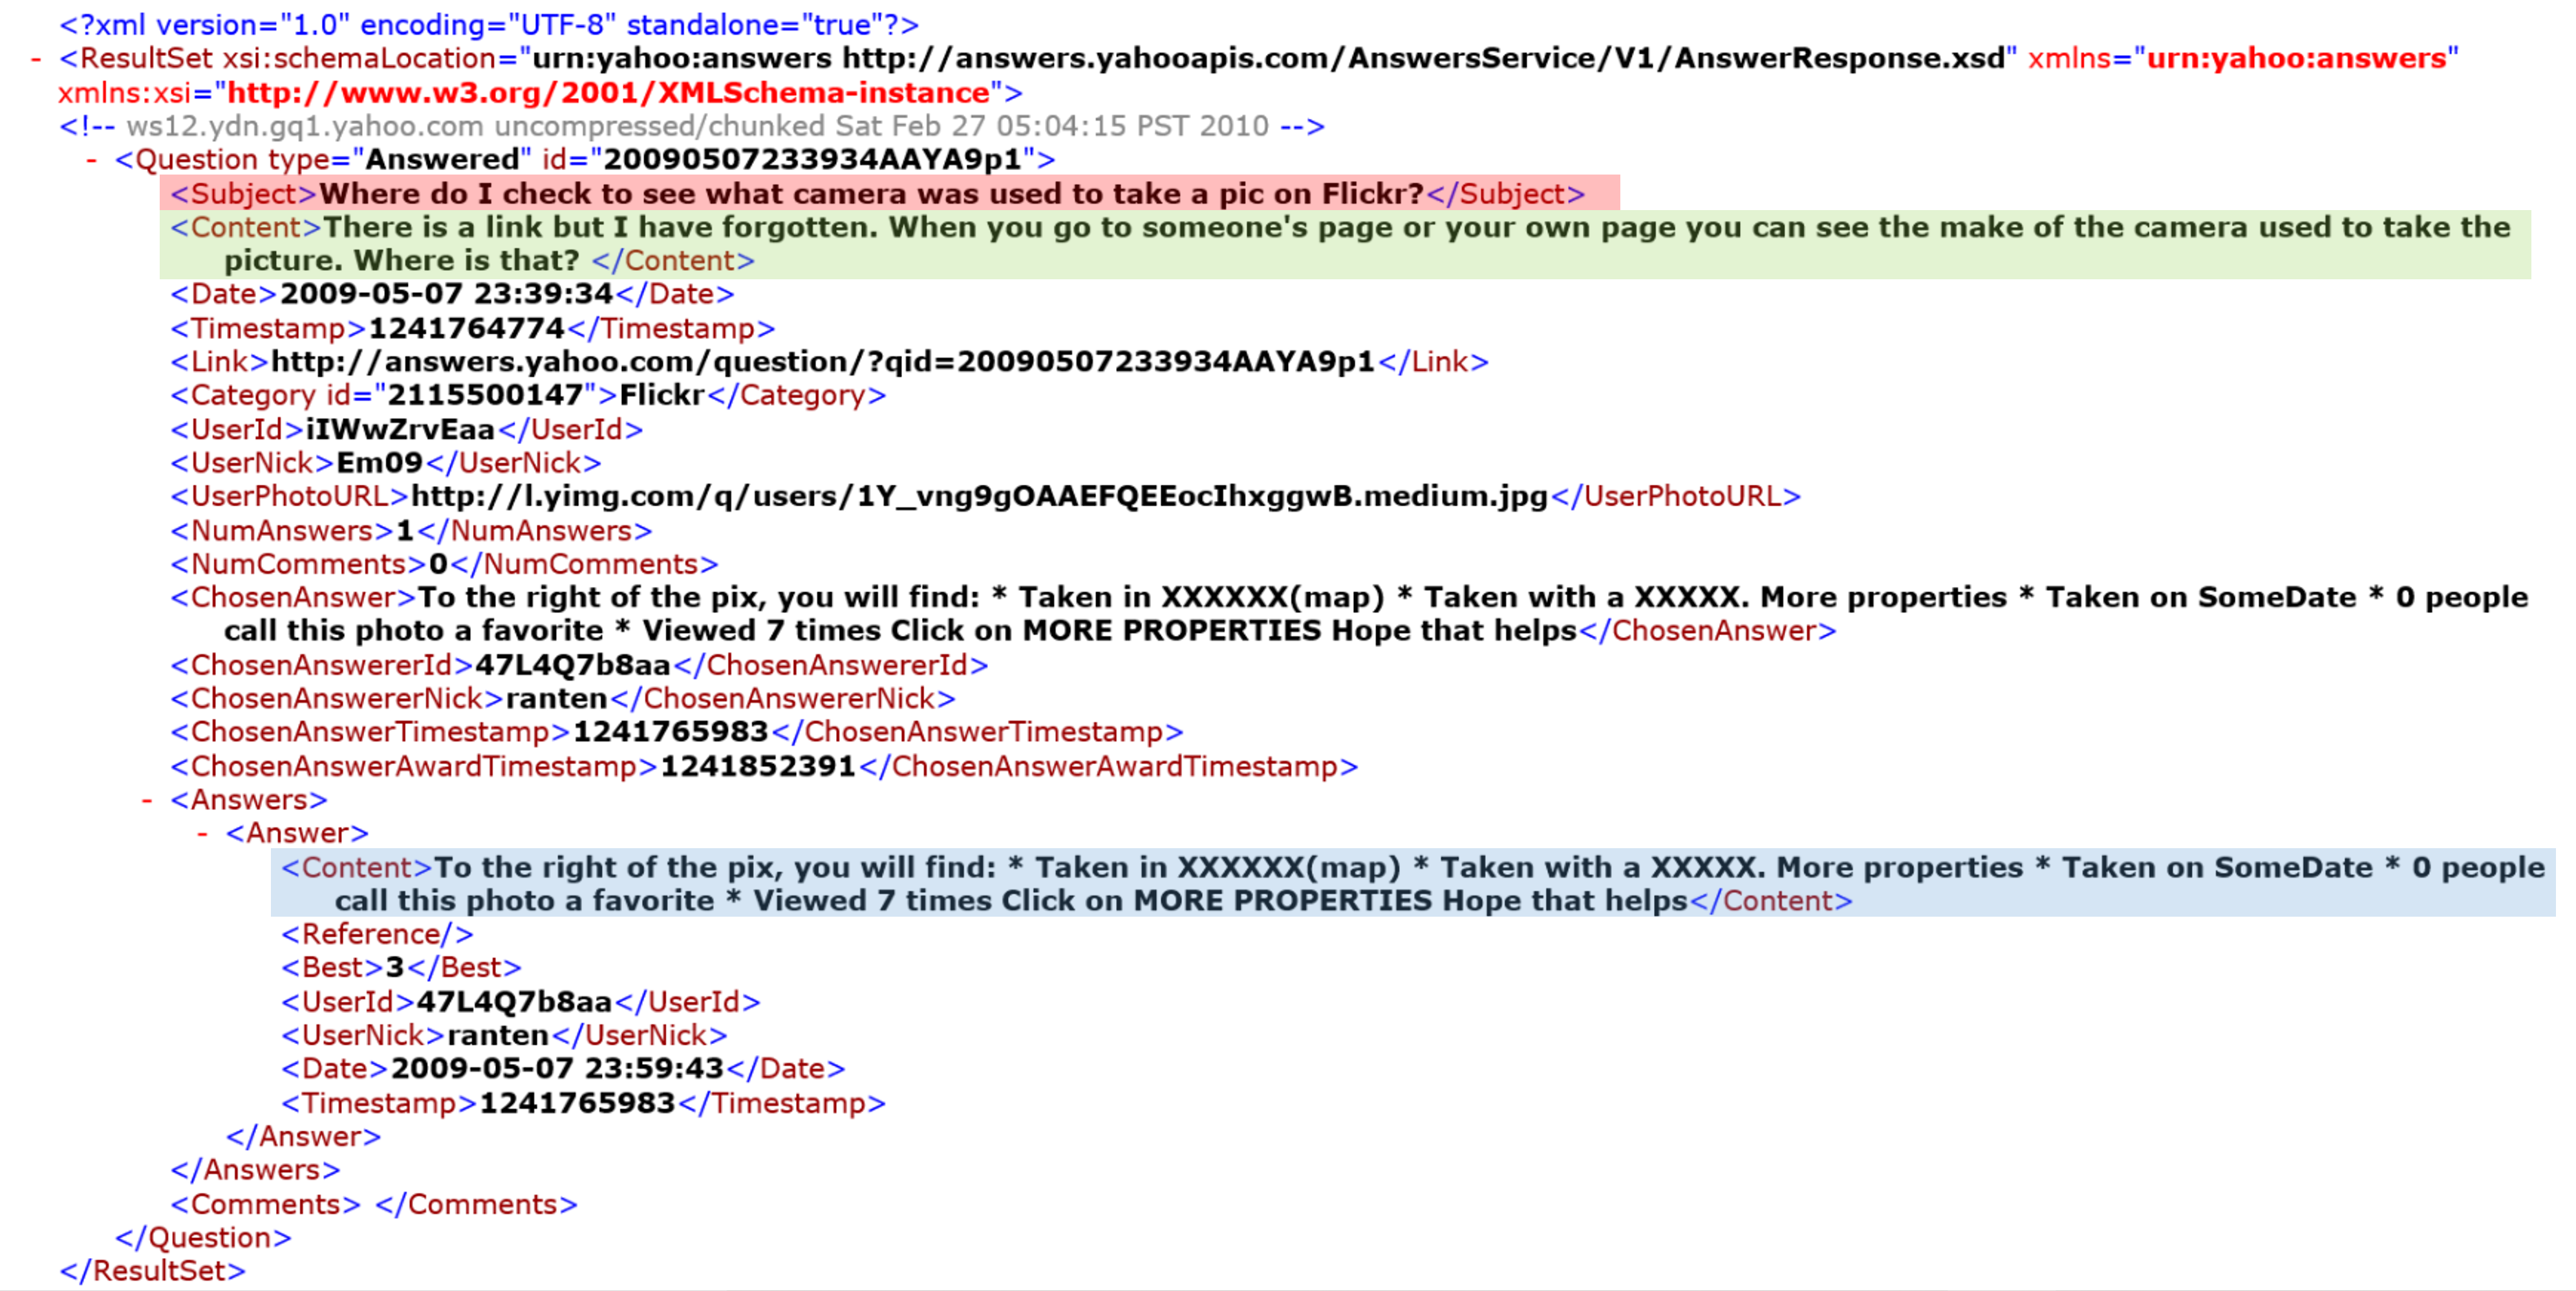
\includegraphics[scale=0.37]{xmlfileeg.png} 
        \centering 
        \caption{.xml file with main branches marked}
        \centering
    \end{figure} 
    \item questions.txt : Contains the details of each community question, the three columns correspond to category, question ID and issue time respectively 
    
    \begin{figure}[h]
        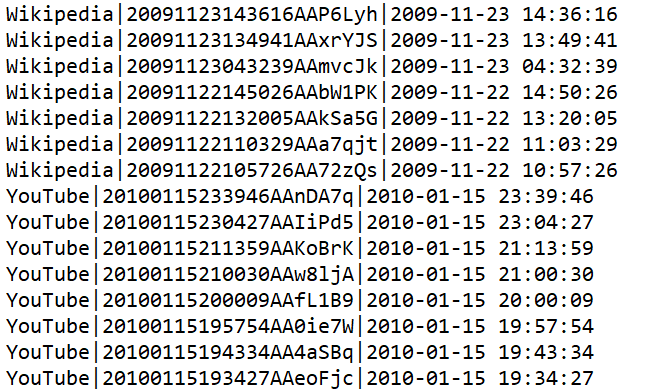
\includegraphics[scale=0.5]{questionstxt.png} 
        \centering 
        \caption{questions.txt}
        \centering
    \end{figure} 
\end{enumerate} 

Each question involves a question subject, question content and answers as branches of the .xml files. The question subject is the actual question itself while the question content is additional information the asker may provide, that does not change the question subject significantly. The answers are a set of 1 or more answers, each ranked by the users. A short Python script was written to extract the subject-question-answers triplets from the .xml files and to create a corresponding .csv file that can easily be parsed into a pandas dataframe in the actual cQA implementation. The pseudocode and Python script can be found in the appendix in section 7.2.1. 

\begin{figure}[h]
    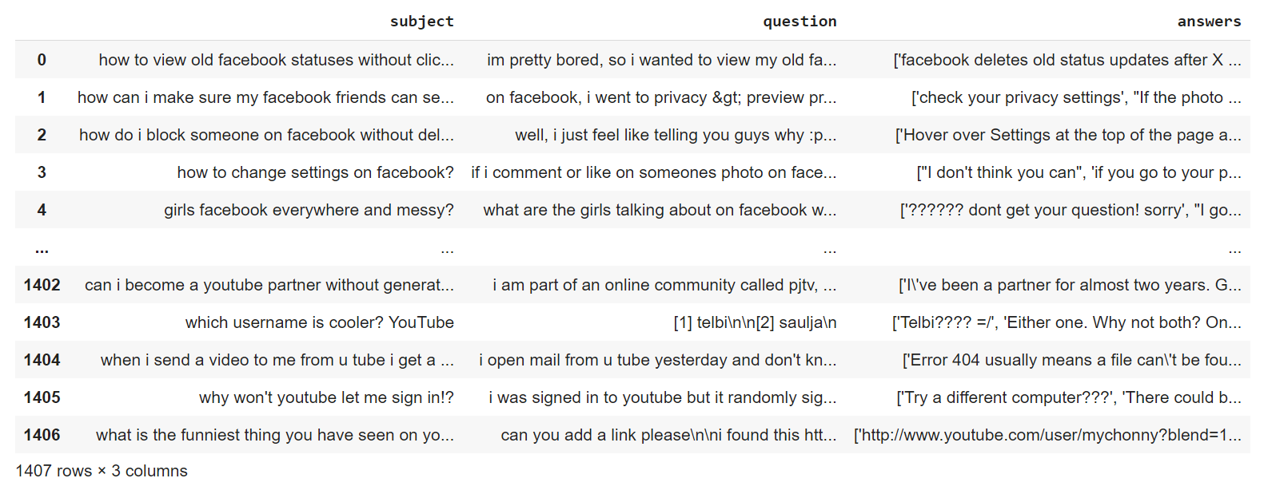
\includegraphics[scale=0.4]{csvsnapshot.png} 
    \centering 
    \caption{Resulting .csv file as loaded into a dataframe}
    \centering 
\end{figure} 

\subsubsection{Dataset 2 : Yahoo! Answers Topic Classification Dataset – 2007} 

This dataset also comprises of question-answer pairs from Yahoo! Answers. It was released by the Yahoo! Research Alliance Webscope Program (2007) and accessed via Kaggle. \cite{dataset2} It was released mainly for classification tasks and each question has a specific class index (10 classes) based on the domain of the question. The test dataset was used here that includes 60000 question-answer pairs. 

\\~\\ 

\begin{center}
  \renewcommand{\arraystretch}{1.5}
  \begin{tabular}{p{2.5cm}|p{5cm}|p{2cm}}
    Class Index&Topic&Number of Questions\\ 
    \hline 
    0&Society \& Culture&6000 \\ 
    1&Science \& Mathematics&6000 \\ 
    2&Health&6000 \\ 
    3&Education \& Reference&6000 \\ 
    4&Computers \& Internet&6000 \\ 
    5&Sports&6000 \\ 
    6&Business \& Finance&6000 \\ 
    7&Entertainment \& Music&6000 \\ 
    8&Family \& Relationships&6000 \\ 
    9&Politics \& Government&6000 \\ 
    \hline
    &&60000 \\  
\end{tabular}
\end{center} 

%\begin{center}
%  \renewcommand{\arraystretch}{1.5}
%  \begin{tabular}{p{2.5cm}|p{5cm}|p{2cm}|p{2cm}}
%    Class Index&Topic&Number of Questions in Original Dataset&Number of Questions Used \\ 
%    \hline 
%    0&Society \& Culture&6000&500 \\ 
%    1&Science \& Mathematics&6000&500 \\ 
%    2&Health&6000&500 \\ 
%    3&Education \& Reference&6000&500 \\ 
%    4&Computers \& Internet&6000&500 \\ 
%    5&Sports&6000&500 \\ 
%    6&Business \& Finance&6000&500 \\ 
%    7&Entertainment \& Music&6000&500 \\ 
%    8&Family \& Relationships&6000&500 \\ 
%    9&Politics \& Government&6000&500 \\ 
%    \hline
%    &&60000&5000 
%\end{tabular}
%\end{center} 

\\~\\ 

\subsection{Framework} 

The suggested framework for the cQA system according to authors Bolanle Ojokoh and Peter Ayokunle is as follows : 

\clearpage
\begin{figure}[h]
    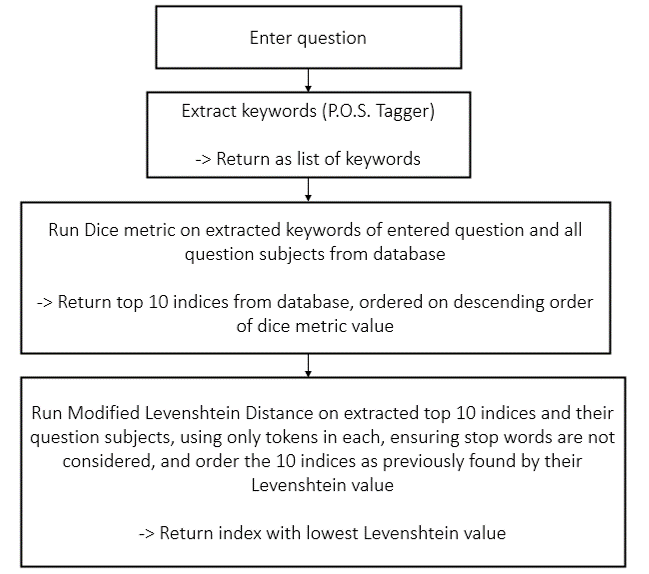
\includegraphics[scale=0.6]{suggested flowchart.png} 
    \centering 
    \caption{Suggested System Pipeline}
    \centering 
\end{figure} 

With this approach, the cQA system performed considerably well but there was scope for improvement. Thus, I first tried multiplying the dice metric and Levenshtein distance after step 4 and using this value instead of just using the Levenshtein distance to rank the question-answer pairs. A few other approaches were also tried, as summarised here : 

\begin{enumerate}
    \item Word-Based Levenshtein Distance with final value as count 
    \item Dice Metric + Word-Based Levenshtein Distance with final value as count 
    \item Dice Metric + Word-Based Levenshtein Distance with final value as count \(\times\) dice metric 
    \item Cosine Similarity alone 
    \item Cosine Similarity + Word-Based Levenshtein Distance with final value as count 
    \item Cosine Similarity + Word-Based Levenshtein Distance final value as count \(\times\) dice metric
\end{enumerate}

\subsection{Evaluation Metrics} 

The main metrics for evaluation in Machine Learning and Information Retrieval are precision and recall. 
\\~\\ 
In the field of machine learning, they are defined as : 
\\~\\ 
Precision = \(\frac{TP}{TP\; +\; FP}\) 
\\~\\ 
Recall = \(\frac{TP}{TP\; +\; FN}\) 
\\~\\ 
where \\ 
TP = True Positives, \\ 
FP = False Positives, \\ 
FN = False Negatives 
\\~\\~\\ 
In the field of IR, they are defined as \cite{precrec}: 
\\~\\
Precision = \(\frac{Number\; of\; (Relevant\; documents\; \cap\; Retrieved\; documents)}{Number\; of\; retrieved\; documents}\) 
\\~\\ 
Recall = \(\frac{Number\; of\; (Relevant\; documents\; \cap\; Retrieved\; documents)}{Number\; of\; relevant\; documents}\) 
\\~\\~\\ 
Since the system implemented does not classify objects, in which case the true positive/false positive metric could be easily used, and the system does not also return lists of documents but only returns one (viewing each question-answer pair as a document), modified versions of the above evaluation metrics better suited to the project were used. The following evaluation metrics \cite{evmets} were used to analyse the cQA system developed : 

\begin{enumerate}
    \item Accuracy = \(\frac{Number\; of\; correctly\; retrieved\; question-answer\; pairs}{Total\; number\; of\; question-answer\; pairs}\) 
    \item Precision = \(\frac{Number\; of\; shared\; words\; between\; prediction\; and\; true\; answer\;}{Total\; number\; of\; words\; in\; prediction\;}\) 
    \item Recall = \(\frac{Number\; of\; shared\; words\; between\; prediction\; and\; true\; answer}{Total\; number\; of\; words\; in\; true\; answer}\) 
    \item F-Score = \(2\times\frac{Precision\; \times \; Recall}{Precision\; +\; Recall}\)
\end{enumerate} 

\newpage 
\subsection{Evaluation Results} 

The same word subjects were passed to the evaluating function and the returned question-answer pairs were compared with the questions passed to analyse the different approaches. This was done for both datasets successively.  
\\~\\~\\ 
Evaluation on Dataset 1 : 
\begin{center}
  \renewcommand{\arraystretch}{1.5}
  \begin{tabular}{p{5.5cm}|c|c|c|c}
    Approach&Accuracy&Precision&Recall&F-Score \\ 
    \hline 
    Word-Based Levenshtein Distance with final value as count&0.95949&0.96238&0.96304&0.96271 \\
    Dice Metric + Word-Based Levenshtein Distance with final value as count&0.93817&0.94215&0.94312&0.94263 \\ 
    Dice Metric + Word-Based Levenshtein Distance with final value as count x dice metric&0.97656&0.97808&0.97779&0.97794 \\ 
    Cosine Similarity alone&0.99787&0.99807&0.99806&0.99807 \\
    Cosine Similarity + Word-Based Levenshtein Distance with final value as count&0.93888&0.94337&0.94445&0.94391 \\ 
    Cosine Similarity + Word-Based Levenshtein Distance with final value as count x dice metric&0.99858&0.99875&0.99876&0.99875 \\ 
\end{tabular} 
\end{center} 

\clearpage 
Evaluation on Dataset 2 : 
\begin{center}
  \renewcommand{\arraystretch}{1.5}
  \begin{tabular}{p{5.5cm}|c|c|c|c}
    Approach&Accuracy&Precision&Recall&F-Score \\ 
    \hline 
    Word-Based Levenshtein Distance with final value as count&0.9816&0.98221&0.98324&0.98272 \\ 
    Dice Metric + Word-Based Levenshtein Distance with final value as count&0.9716&0.97272&0.97369&0.9732 \\ 
    Dice Metric + Word-Based Levenshtein Distance with final value as count x dice metric&0.984&0.9847&0.98466&0.98468 \\ 
    Cosine Similarity alone&0.9978&0.99803&0.99802&0.99802 \\
    Cosine Similarity + Word-Based Levenshtein Distance with final value as count&0.9746&0.97576&0.97746&0.97661 \\
    Cosine Similarity + Word-Based Levenshtein Distance with final value as count x dice metric&0.9986&0.99873&0.99878&0.99875 \\ 
\end{tabular}
\end{center} 
\\~\\~\\~\\ 
The F-scores for both datasets per approach were averaged to get a resultant F-score as representative of the system as a whole. 

\clearpage
Average F-Scores : 
\begin{center}
  \renewcommand{\arraystretch}{1.5}
  \begin{tabular}{p{5cm}|p{2.5cm}|p{2.5cm}|p{2.5cm}}
    Approach&F-Scores for Dataset 1&F-Scores for Dataset 2&Average F-Score across datasets \\ 
    \hline 
    Word-Based Levenshtein Distance with final value as count&0.96271&0.98272&\textbf{0.972715} \\ 
    Dice Metric + Word-Based Levenshtein Distance with final value as count&0.94263&0.9732&\textbf{0.957915} \\ 
    Dice Metric + Word-Based Levenshtein Distance with final value as count x dice metric&0.97794&0.98468&0.98131 \\ 
    Cosine Similarity alone&0.99807&0.99802&0.998045 \\ 
    Cosine Similarity + Word-Based Levenshtein Distance with final value as count&0.94391&0.97661&0.96026 \\ 
    Cosine Similarity + Word-Based Levenshtein Distance with final value as count x dice metric&0.99875&0.99875&\textbf{0.99875} \\  
\end{tabular}
\end{center} 
\\~\\~\\ 
As can be seen, the best performance is observed for \textbf{approach 6 (Cosine Similarity + Word-Based Levenshtein Distance with final value as count \(\times\) dice metric)} with an F-Score of \textbf{0.99875}. The worst performance is observed for \textbf{approach 2 (Dice Metric + Word-Based Levenshtein Distance with final value as count)}. The approach followed in the paper referred to \cite{maincqa} i.e. approach 2  gave an F-Score of \textbf{0.957915} as compared to the F-Score 0f 0.951 achieved in the paper. \textbf{Approach 1 (Word-Based Levenshtein Distance with final value as count)} gave an F-Score of \textbf{0.972715} as compared to the F-Score of 0.934 achieved in the paper \cite{maincqa}. 

\newpage 
\section{Conclusions} 

The cQA system that was implemented as part of this project had 6 different approaches to the problem. The best performing approach was the approach that used cosine similarity and Levenshtein distance and ranked question-answer pairs based on the value obtained by multiplying both the above text similarity measures. The achieved F-Score was \textbf{0.99875} on both datasets combined, thus performing \textbf{1.05} (0.99875/0.951) times better than the reference paper. 
\\~\\ 
The approaches can be ranked as follows based on their F-Scores : 
\\~\\ 
\textbf{1} \(\rightarrow\) Cosine Similarity + Word-Based Levenshtein Distance with final value as count \(\times\) dice metric \\ 
\textbf{2} \(\rightarrow\) Cosine Similarity alone \\ 
\textbf{3} \(\rightarrow\) Dice Metric + Word-Based Levenshtein Distance with final value as count \(\times\) dice metric \\ 
\textbf{4} \(\rightarrow\) Word-Based Levenshtein Distance with final value as count \\ 
\textbf{5} \(\rightarrow\) Cosine Similarity + Word-Based Levenshtein Distance with final value as count \\ 
\textbf{6} \(\rightarrow\) Dice Metric + Word-Based Levenshtein Distance with final value as count \\ 


\section{Further Research} 

For the open-domain Wiki QA system, as mentioned before, passage retrieval methods like BM25 and DPR will be tried out instead of Cosine Similarity in an attempt to improve performance. The Roberta-Base pretrained model will also be modified by adding layers and finetuning. NLG (natural language generation) will also be tried out instead of SQuAD answer extraction. 
\\~\\ 
For the cQA system, the main focus of this project, further research will be carried out on text similarity measures. Jaccard metric, K Means, Jensen Shannon distance and other such measures will also be tried out and their performance compared with the best that has been achieved yet with cosine similarity and word-based Levenshtein distance, and methods like posterior regularisation will also be implemented \cite{postreg}. More datasets of question-answer pairs will also be used to test the system and run further evaluations. 

\newpage 
\section{Appendix} 
\subsection{Standard QA System} 

\begin{lstlisting}[language = Python] 
## Imports

# General downloads
!pip install transformers datasets
!pip install wptools
!pip install wikipedia 

import itertools 
import os 
import numpy 
import re 

# HuggingFace Transformers
from transformers import AutoTokenizer, 
    AutoModelForQuestionAnswering, pipeline 
import tensorflow as tf
import spacy 

import nltk 
nltk.download('wordnet')
nltk.download('punkt')
nltk.download('averaged_perceptron_tagger') 

# MediaWiki API 
import wptools 
import wikipedia 

from sklearn.feature_extraction.text 
    import TfidfVectorizer
from sklearn.metrics.pairwise import cosine_similarity 
from sklearn.metrics.pairwise import linear_kernel

# Model trained on the SQuAD 2.0 dev set 
model_name = "deepset/roberta-base-squad2"

qa_final = pipeline('question-answering', model = 
    model_name, tokenizer = model_name)

## Modules

def getKeywords(question): 
    tagged = nltk.pos_tag(nltk.word_tokenize(question)) 
    print(tagged) 

    # The NLTK POS Tagger follows the Penn Treebank 
    # Project tag conventions 
    # Only the following kinds of words are extracted 
    # from the query as keywords 
    limit = ['FW', 'JJ', 'JJS', 'JJR', 'NN', 'NNS', 
        'NNP', 'NNPS', 'SYM'] 
    keywords = ' '.join(i[0] for i in tagged if i[1] 
        in limit) 
    print(keywords) 
    return keywords

def retrieveDocs(keywords): 
    wiki_search = wikipedia.search(keywords) 
    print("Wiki search results:") 
    print(wiki_search) 
    print("\n" + '='*(20) + "\n")
    documents = []
    documentTitles = []
    for i in wiki_search: 
        page = wptools.page(str(i))
        page.get_parse() 
        # print(str(i), page.data['pageid']) 
        try: 
            content = wikipedia.page(pageid = 
                page.data['pageid']) 
        except: 
            continue
        documentTitles.append(str(i))
        res = cleanDoc(content.content)
        documents.append(res) 
    print("Entries considered:") 
    print(documentTitles) 
    print("\n" + '='*(20) + "\n")
    return documents

def cleanDoc(content):
      headings_to_remove = ['== Further reading ==', 
        '== Further references ==', 
        '=== Citations ===', '== References ==', 
        '== Footnotes ==', '=== Notes ===','== Notes ==', 
        '=== Sources ===', '== Sources ==', 
        '== External links', '== See also ==', ]
      
      headings_to_remove = '|'.join(headings_to_remove) 
      inds = [m.start() for m in 
        re.finditer(headings_to_remove, content)]
      # print(inds) 
      if len(inds) != 0: 
          mini = min(inds) 
          mini = min(mini, len(content)) 
      else: 
          mini = len(content)
      # print(mini)
      return content[:mini]

def splitDocs(question, documents): 
    passages = [question]
    for i in documents: 
        curr_passages = [p for p in i.split('\n') if p 
            and not p.startswith('=')] 
        passages += curr_passages 
    return passages

def retrievePassages(question, documents): 
    passages = {}
    for i in documents: 
        curr_passages = [p for p in i.split('\n') if p 
            and not p.startswith('=')] 
        curr_passages.insert(0, question) 
        tfidf = TfidfVectorizer().fit_transform
            (curr_passages) 
        cosSims = linear_kernel(tfidf[0:1], 
            tfidf).flatten() 
        curr_passages = dict(zip(curr_passages, 
            cosSims)) 
        curr_passages = dict(sorted(curr_passages.items(), 
            key = lambda item: item[1], reverse = True)) 
        p = list(curr_passages.keys()) 
        s = list(curr_passages.values()) 
        i = 1 
        while i < len(p) and i < 10: 
          passages[p[i]] = s[i] 
          i += 1

    print(passages) 
    passages = dict(sorted(passages.items(), 
        key = lambda item: item[1], reverse = True)) 
    print(passages.values())
    passages = list(passages.keys())[:10] 
    print(passages) 
    return passages

def printRelevantPassages(passages): 
    print("Most relevant passages: ")
    for i in passages: 
        print(i) 
    print("\n" + '='*(20) + "\n")

def getAnswers(question, passages): 
    possibleAnswers = []
    for i in passages: 
        possibleAnswers.append(qa_final(question = 
            question, context = i)) 
    # print(possibleAnswers) 
    possibleAnswers = sorted(possibleAnswers, 
        key = lambda i: i['score']) 
    return possibleAnswers

def printAllAnswers(possibleAnswers): 
    print("Possible answers sorted by confidence rating: ")
    for i in range(len(possibleAnswers) - 1, -1, -1): 
        print(str(len(possibleAnswers) - 1 - i + 1) + 
            '.' + possibleAnswers[i]['answer'] + ':' + 
            str(possibleAnswers[i]['score'])) 
    print("\n" + '='*(20) + "\n")

## System

##### 
# Type either keywords only or the entire question itself 
# No yes/no questions 
#####

question = input("Enter question: ")

keywords = getKeywords(question) 
documents = retrieveDocs(keywords) 
passages = retrievePassages(question, documents) 
printRelevantPassages(passages) 
possibleAnswers = getAnswers(question, passages) 
printAllAnswers(possibleAnswers)

print(question) 
print(possibleAnswers[-1]['answer']) 
\end{lstlisting}

\subsection{cQA System} 
\subsubsection{Dataset 1 : Yahoo! Answers Dataset for cQA – 2010} 


\textbf{Pseudocode : }
\begin{enumerate}
    \item Read questions.txt line by line 
    \item For each question ID, read corresponding xml file 
    \item Extract data under \(<\)Subject\(>\) and \(<\)Content\(>\) 
    \item Split \(<\)Content\(>\) into one string for question (always the first string in returned array) and the rest of the array (may or may not be singleton) as possible answers 
    \item Write Subject, Question Content and Answer(s) to csv 
\end{enumerate}
\\~\\
\textbf{Dependency : } 
BeautifulSoup xml reader 
\\~\\
\textbf{Script : } 
\begin{lstlisting}[language = Python]
import csv 
from bs4 import BeautifulSoup 

row = ['subject', 'question', 'answers']
wd = [] 
wd.append(row)
# with open('cqa.csv', 'w', encoding = 'UTF8', 
    newline = '') as h: 
#     writer = csv.writer(h) 
#     writer.writerow(row)

f = open('questions.txt', 'r') 
for x in f: 
    sp = x.split('|') 
    fn = sp[1] + '.xml' 
    
    with open(fn, 'r', encoding = "utf8") as g:
        data = g.read() 
    bs_data = BeautifulSoup(data, 'xml') 

    row = []
    sub = str(bs_data.find('Subject'))[9:-10].lower()
    if sp[0].lower() not in sub: 
        sub += ' ' + sp[0]
    row.append(sub) 
    con = bs_data.find_all('Content')
    for i in range(len(con)): 
        con[i] = str(con[i])[9:-10]
    row.append(con[0].lower()) 
    row.append(con[1:]) 
    print("*****")
    print(row[0]) 
    print(row[1]) 
    print(row[2]) 
    wd.append(row)

with open('cqa.csv', 'w', encoding = 'UTF8', newline = '') as h: 
    writer = csv.writer(h) 
    writer.writerows(wd) 
\end{lstlisting}


\subsubsection{Implementation} 

\begin{lstlisting}[language = Python]
## Imports 

import itertools
import os 
import string 

import matplotlib.pylab as plt 
from matplotlib import pyplot
import numpy as np 
import pandas as pd 

import tensorflow as tf

import random 
import re
import nltk 
nltk.download('wordnet')
nltk.download('punkt')
nltk.download('averaged_perceptron_tagger') 

from nltk.corpus import stopwords
nltk.download('stopwords') 
from nltk.tokenize import word_tokenize
from nltk.stem.lancaster import LancasterStemmer
lancaster_stemmer = LancasterStemmer()
from nltk.stem import WordNetLemmatizer
wordnet_lemmatizer = WordNetLemmatizer() 

from sklearn.feature_extraction.text 
    import TfidfVectorizer
from sklearn.metrics.pairwise import cosine_similarity 
from sklearn.metrics.pairwise import linear_kernel

## Modules

qa_pairs1 = pd.read_csv('cqa.csv', sep=',', header=0, 
    encoding="utf-8") #Dataframe

qa_pairs1

qa_pairs_l1 = qa_pairs1.values.tolist()

qa_pairs2 = pd.read_csv('test.csv', sep=',', header=0, 
    encoding="utf-8") #Dataframe

del qa_pairs2["class index"]

qa_pairs2

qa_pairs_l2 = qa_pairs2.values.tolist()

qa_pairs_ext = [] 
for i in range(10): 
  qa_pairs_ext += qa_pairs_l2[i * 6000:i * 6000 + 500]

def getKeywords(question): 
    tagged = nltk.pos_tag(nltk.word_tokenize(question)) 
    print(question)
    print(tagged) 

    # The NLTK POS Tagger follows the Penn Treebank 
    # Project tag conventions 
    # Only the following kinds of words are extracted 
    # from the query as keywords 
    limit = ['FW', 'JJ', 'JJS', 'JJR', 'NN', 'NNS', 'NNP', 
        'NNPS', 'SYM', 'VB'] 
    keywords = [i[0] for i in tagged if i[1] in limit]
    print(keywords) 
    return keywords

def cosSim(question, qa_pairs_l): 
  res = {}
  subs =[]
  for i in range(len(qa_pairs_l)): 
    subs.append(qa_pairs_l[i][0])
  subs.insert(0, question) 
  tfidf = TfidfVectorizer().fit_transform(subs) 
  cosSims = linear_kernel(tfidf[0:1], tfidf).flatten() 
  i = 1 
  while i < len(subs): 
    subs[i] = i - 1 
    i += 1 
  subs = dict(zip(subs, cosSims)) 
  subs = dict(sorted(subs.items(), key = lambda item: 
    item[1], reverse = True)) 
  # print(subs)
  subsk = list(subs.keys()) 
  subsv = list(subs.values()) 
  i = 1 
  while i < 10: 
    res[subsk[i]] = subsv[i] 
    i += 1 
  res = sorted(res.items(), key = lambda i: i[1], 
    reverse = True) 
  return res

def diceMetric(keywords, qa_pairs_l, ql): 
  res = {}
  for i in range(len(qa_pairs_l)): 
    count = 0 
    for j in keywords: 
      if j in qa_pairs_l[i][0]: 
        count += 1 
    count *= 2 
    count /= (ql + len(qa_pairs_l[i][0])) 
    res[i] = count 
  res = sorted(res.items(), key = lambda i: i[1]) 
  res = res[::-1]
  return res[:10]

stop_words = set(stopwords.words('english'))
if "the" in stop_words: 
  print("Yes")

def levenshtein(question, res, qa_pairs_l): 
  qc = question.translate
    (str.maketrans('', '', string.punctuation)) 
  tq = qc.split(" ")
  fin = {}
  for i in res: 
    curr = qa_pairs_l[i[0]][0].translate
        (str.maketrans('', '', string.punctuation)) 
    tcurr = curr.split(" ") 
    count = 0 
    for j in tq: 
      if j not in stop_words and j in tcurr: 
        count += 1 
    fin[i[0]] = count * i[1] 
    # fin[i[0]] = count 
  fin = sorted(fin.items(), key = lambda i: i[1]) 
  # print(fin)
  return fin[-1][0] 
  # return fin[0][0]

def levenshtein_mod(question, res, qa_pairs_l): 
  qc = question.translate
    (str.maketrans('', '', string.punctuation)) 
  tq = qc.split(" ")
  fin = {}
  for i in range(len(res)): 
    curr = qa_pairs_l[i][0].translate
        (str.maketrans('', '', string.punctuation)) 
    tcurr = curr.split(" ") 
    count = 0 
    for j in tq: 
      if j not in stop_words and j in tcurr: 
        count += 1 
    fin[i] = count
  fin = sorted(fin.items(), key = lambda i: i[1]) 
  # print(fin)
  return fin[-1][0] 
  # return fin[0][0] 

def encaps(question, qa_pairs_l): 
  keywords = getKeywords(question) 
  ql = len(question) 
  
  # Only Levenstein with count
  # ind = levenshtein_mod(question, qa_pairs_l, qa_pairs_l) 

  # Dice + Levenshtein without mult 
  # d = diceMetric(keywords, qa_pairs_l, ql) 
  # stop_words = set(stopwords.words('english')) 
  # ind = levenshtein(question, d, qa_pairs_l) 
  # Reverse fin lines

  # Dice + Levenshtein with mult 
  # d = diceMetric(keywords, qa_pairs_l, ql) 
  # stop_words = set(stopwords.words('english')) 
  # ind = levenshtein(question, d, qa_pairs_l) 

  # CosSim only 
  # ind = cosSim(question, qa_pairs_l) 

  # CosSim + Levenshtein without mult 
  # c = cosSim(question, qa_pairs_l) 
  # ind = levenshtein(question, c, qa_pairs_l) 
  # Reverse fin lines 

  # CosSim + Levenshtein with mult 
  c = cosSim(question, qa_pairs_l) 
  ind = levenshtein(question, c, qa_pairs_l) 
  
  # print(qa_pairs_l[ind])
  return ind 

def eval(qa_pairs_l): 
  count = 0 
  for i in range(len(qa_pairs_l)): 
    q = qa_pairs_l[i][0]
    ans = encaps(q, qa_pairs_l) 
    if qa_pairs_l[ans][0] == q: 
      count += 1 
  ratio = count / len(qa_pairs_l) 
  return ratio

def eval_mod(qa_pairs_l): 
  precision = 0 
  recall = 0 
  for i in range(len(qa_pairs_l)): 
    q = qa_pairs_l[i][0]
    ans = encaps(q, qa_pairs_l) 
    if qa_pairs_l[ans][0] == q: 
      precision += 1 
      recall += 1 
    else: 
      shared = 0 
      qset = list(set(q.split(" "))) 
      ansset = list(set(qa_pairs_l[ans][0].split(" ")))
      for j in qset: 
        if j in ansset: 
          shared += 1 
      # print(shared / len(qa_pairs_l[ans][0]), i)
      precision += shared / len(qa_pairs_l[ans][0]) 
      recall += shared / len(q) 
  precision /= len(qa_pairs_l) 
  recall /= len(qa_pairs_l) 
  print(precision, recall) 
  fscore = 2 * (precision * recall) / (precision + recall) 
  return fscore

eval(qa_pairs_l1) 

eval_mod(qa_pairs_l1) 

eval(qa_pairs_ext)

eval_mod(qa_pairs_ext) 
\end{lstlisting}

\newpage 
\section{References}
% \nocite{*} 
\bibliographystyle{plain} 
\bibliography{refs} 
\end{document}
